%----------------------------------------------------------------------------------------
%	PACKAGES AND OTHER DOCUMENT CONFIGURATIONS
%----------------------------------------------------------------------------------------

\documentclass[11pt]{scrartcl} % Font size

\input{structure.tex} % Include the file specifying the document structure and custom commands
\usepackage{multirow}
\usepackage{array}
\usepackage{subcaption}
% Bar chart drawing library 
\usepackage{pgfplots} 
\usepackage{textcomp}

% Define a macro to create a table with fixed column widths
\newcolumntype{C}[1]{>{\centering\arraybackslash}p{#1}}

\usepackage{hyperref}
\hypersetup{
    colorlinks=true,
    linkcolor=blue,
    filecolor=magenta,      
    urlcolor=cyan,
}

\definecolor{codegreen}{rgb}{0,0.6,0}
\definecolor{codegray}{rgb}{0.5,0.5,0.5}
\definecolor{codepurple}{rgb}{0.58,0,0.82}
\definecolor{backcolour}{rgb}{0.95,0.95,0.92}
\definecolor{codeblue}{rgb}{0,0,0.8}

\lstdefinestyle{mystyle}{
    backgroundcolor=\color{backcolour},   
    commentstyle=\color{codegreen},
    keywordstyle=\color{codeblue},
    numberstyle=\tiny\color{codegray},
    stringstyle=\color{codepurple},
    basicstyle=\ttfamily\footnotesize,
    breakatwhitespace=false,         
    breaklines=true,                 
    captionpos=b,                    
    keepspaces=true,                 
    numbers=left,                    
    numbersep=5pt,                  
    showspaces=false,                
    showstringspaces=false,
    showtabs=false,                  
    tabsize=2
}

\lstset{style=mystyle}

\newcommand{\showpcaimage}[1]{
    \begin{figure}[H]
        \centering
        \begin{subfigure}[b]{0.45\textwidth}
            \includegraphics[width=\textwidth]{./assets/#1_1.jpg}
            \caption{Ποσοστό από Principal Components -- 1\%}
        \end{subfigure}
        \begin{subfigure}[b]{0.45\textwidth}
            \includegraphics[width=\textwidth]{./assets/#1_25.jpg}
            \caption{Ποσοστό από Principal Components -- 25\%}
        \end{subfigure}
        \begin{subfigure}[b]{0.45\textwidth}
            \includegraphics[width=\textwidth]{./assets/#1_75.jpg}
            \caption{Ποσοστό από Principal Components -- 75\%}
        \end{subfigure}
        \begin{subfigure}[b]{0.45\textwidth}
            \includegraphics[width=\textwidth]{./assets/#1_100.jpg}
            \caption{Ποσοστό από Principal Components -- 100\%}
        \end{subfigure}
        \caption{Ποσοστό από Principal Components που κρατήσαμε. Εικόνα \src{#1}}
    \end{figure}
}

%----------------------------------------------------------------------------------------
%	TITLE SECTION
%----------------------------------------------------------------------------------------

\title{	
	\normalfont\normalsize
	\textsc{Πανεπιστήμιο Πατρών, Τμήμα Μηχανικών ΗΥ και Πληροφορικής}\\ % Your university, school and/or department name(s)
	\vspace{25pt} % Whitespace
	\rule{\linewidth}{0.5pt}\\ % Thin top horizontal rule
	\vspace{20pt} % Whitespace
    {\LARGE Λογισμικό και Προγραμματισμός Συστημάτων Υψηλής Επίδοσης\\ Άσκηση 3 - CUDA \& OpenACC}\\ % The assignment title
	\vspace{12pt} % Whitespace
	\rule{\linewidth}{2pt}\\ % Thick bottom horizontal rule
	\vspace{12pt} % Whitespace
}


\author{Ευάγγελος Λάμπρου \\UP1066519 \and Ιωάννης Παναρίτης \\UP1072632} % Your name

\date{} % Today's date (\today) or a custom date

%----------------------------------------------------------------------------------------
%	DOCUMENT
%----------------------------------------------------------------------------------------

\bibliographystyle{abbrv}
\addto\captionsgreek{\renewcommand{\refname}{Αναφορές}}

\begin{document}

\maketitle 

\section{CUDA}

\subsection{Υλοποίηση}

Για την υλοποίηση αυτής της άσκησης έγινε \say{μετάφραση} του κώδικα Matlab σε C++.
Βασική διαφορά είναι η χρήση της βιβλιοθήκης Lapack για τις πράξεις γραμμικής άλγεβρας (υπολογισμός ιδιοτιμών/ιδιοδιανυσμάτων, πολλαπλασιασμός πινάκων).

Με OMP έχουμε παραλληλοποιήσει τα βήματα του PCA όπως: 

\begin{itemize}
    \item Υπολογισμός mean/std 
    \item Normalization
    \item Υπολογισμός του Covariance Matrix.
    \item Επιλογή των $k$ Principal Components.
\end{itemize}

\subsection{Μετρήσεις}

Οι παρακάτω μετρήσεις έγιναν σε σύστημα με επεξεργαστή \src{AMD Ryzen 7 2700 Eight-Core Processor @ 3.20 GHz} και κάρτα γραφικών \src{NVIDIA GeForce GTX 1660 6GB}.

% \begin{table}[H]
%     \centering
%     \begin{tabular}{|l|l|l|}
%     \hline
%         \textbf{Implementation} & \textbf{N} & \textbf{Time (s)} \\ \hline
%         \src{diffusion\_serial}  &  1024    & 22.1073 \\ \hline 
%         \src{diffusion\_cuda} 	 &  1024    & 2.76905 \\ \hline
%         \src{diffusion\_serial}  &  2048    & 367.739 \\ \hline
%         \src{diffusion\_cuda}    &  2048    & 43.6307 \\ \hline
%     \end{tabular}
%     \caption{Χρόνοι εκτέλεσης της υλοποίηση με και χωρίς CUDA.}
% \end{table}

% create a bar plot of the above time measurements using tikz. make it a centered figure with a caption.
\begin{figure}[H]
    \begin{center}
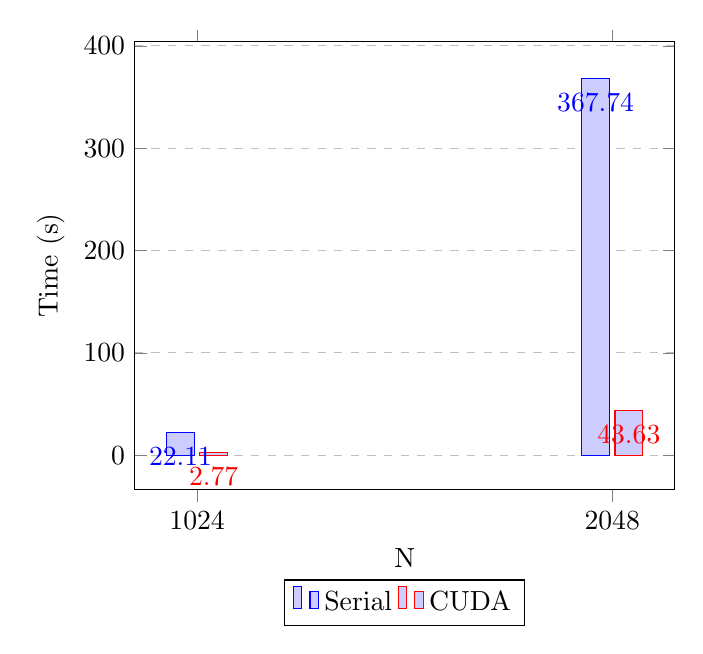
\begin{tikzpicture}
    \begin{axis}[
        xlabel={N},
        ylabel={Time (s)},
        xtick=data,
        xticklabels={1024, 2048},
        ybar,
        enlarge x limits=0.15,
        bar width=10pt,
        legend style={at={(0.5,-0.20)}, anchor=north, legend columns=-1},
        legend entries={Serial, CUDA},
        ymajorgrids=true,
        y grid style=dashed,
        nodes near coords,
        nodes near coords align={vertical},
        nodes near coords style={anchor=north},
        every node near coord/.append style={yshift=-2pt},
        every axis plot post/.append style={fill=blue!20},
        ]
        \addplot coordinates {(1024, 22.1073) (2048, 367.739)};
        \addplot coordinates {(1024, 2.76905) (2048, 43.6307)};
    \end{axis}
\end{tikzpicture}
    \end{center}
    \caption{Χρόνοι εκτέλεσης της υλοποίηση με και χωρίς CUDA.}
    \label{fig:cuda_times}
\end{figure}



{\ttfamily
\lstinputlisting{assets/passed.txt}
}

\subsection{Έλεγχος Αποτελεσμάτων}

\section{OpenACC}

\subsection{Υλοποίηση}

Για την υλοποίηση αυτής της άσκησης αρχικά δημιουργήσαμε μία 
βασική υλοποίηση της προσομοίωσης μυρμηγκιών σε C++.

Με τον perf profiler φαίνεται πως η πλειονότητα του χρόνου σπαταλάται στην συνάρτηση \src{Colony::update},
πράγμα προφανές.

\lstinputlisting[caption=Αποτελέσματα του perf report.]{assets/perf_report.txt}

Στη συνέχεια προστέθηκαν τα directives για την παραλληλοποίηση του κώδικα με την OpenACC.
Σημαντικό ήταν να ελαχιστοποιήσουμε την μεταφορά δεδομένων. Αυτό γίνεται με την χρήση των \src{copyin} και \src{copyout} directives,
όπως και η προσθήκη των \src{present} directives όταν δεδομένα ξέρουμε πως θα βρίσκονται ήδη στην κάρτα γραφικών.

Τελικά στην υλοποίησή έχουμε μία αρχική μεταφορά δεδομένων 
κατά την αρχικοποίηση της κλάσης \src{Collony::Colony} και αποδέσμευση των δεδομένων στην συνάρτηση \src{Collong::{\textasciitilde}Colony}.

\lstinputlisting[caption=Αρχικοποίηση της κλάσης \src{Colony}., language=C++, firstline=31, lastline=47]{assets/colony.cpp}

\lstinputlisting[caption=Καταστροφή της κλάσης \src{Colony}., language=C++, firstline=49, lastline=56]{assets/colony.cpp}

Έτσι, συγχρονίζουμε τα δεδομένα μεταξύ host και device (κάρτα γραφικών) και κατά την παραλληλοποίηση του κώδικα, 
μπορούμε να χρησιμοποίησουμε το \src{kernels} directive χωρίς να γίνεται περαιτέρω μεταφορά δεδομένων.

Τα δεδομένα βρίσκονται μονίμως στην μνήμη της κάρτας γραφικών εκτός από το τέλος της προσομοίωσης, όπου γίνεται μεταφορά των αποτελεσμάτων στο host.

\subsection{Μετρήσεις}
\subsection{Έλεγχος Αποτελεσμάτων}

Για τον έλεγχο των αποτελεσμάτων έγινε συγκρίνοντας 
την τελική κατάσταση του πίνακα των μυρμηγκιών και της φερομόνης 
μεταξύ του σειριακού κώδικα και του παραλληλοποιημένου.

% show terminal output 
\begin{lstlisting}[language=Bash]
$ diff simulation_serial.log simulation_acc.log && echo "Same!"
Same!
\end{lstlisting}

% \bibliography{bibliography}

\end{document}
